\documentclass[10pt,letterpaper]{article}
\usepackage[T1]{fontenc}
\usepackage[utf8]{inputenc}
\usepackage{lmodern,amsmath,amssymb,array,longtable,booktabs,xcolor,titlesec,fancyhdr,hyperref,graphicx,tikz,pgfplots}
\usetikzlibrary{positioning}
\pgfplotsset{compat=1.18}
\usepackage[left=.9in,right=.9in,top=.779861in,bottom=.75in,headsep=.22in]{geometry}
\definecolor{navy}{HTML}{16324F}\definecolor{teal}{HTML}{246A73}
\titleformat{\section}{\sffamily\large\bfseries\color{navy}}{}{0pt}{}
\titleformat{\subsection}{\sffamily\normalsize\bfseries\color{teal}}{}{0pt}{}
\pagestyle{fancy}\fancyhf{}\fancyhead[L]{\sffamily\scriptsize\color{gray}ARWLF | TERNARY SUBSET-SUM ROOT REPORTING}
\fancyfoot[L]{\scriptsize Research draft | revision8e9fe7f}\fancyfoot[R]{\thepage}
\renewcommand{\headrulewidth}{0pt}\setlength{\headheight}{15pt}
\setlength{\parindent}{0pt}\setlength{\parskip}{5pt}\setlength{\emergencystretch}{3em}
\hypersetup{colorlinks=true,urlcolor=teal,linkcolor=navy}
% Standalone: inline bibliography and plots, no external project files needed.
% references.bib is supplied separately for venue-specific BibTeX conversion.
% DOCX retained template is the exact typography/layout authority.
\begin{document}


{\centering\sffamily\fontsize{25}{29}\selectfont\bfseries\color{navy}Cheap Dense Pair Scans with Late Materialization for Ternary Subset-Sum Root Reporting\par}\vspace{8pt}

{\centering\color{teal}A source-derived algorithm-engineering study of the frozen ARWLF backend\par}\vspace{6pt}

Research manuscript draft \textbullet{} Analyzed 3 October 2026 \textbullet{} Author and affiliation metadata reserved for human completion


\subsection*{Abstract}

Ternary Representation Technique (TER) root reporting can produce substantial projected candidate traffic even when no exact root triple survives. We study ARWLF, a frozen arithmetic reporting backend in a classical depth-three TER research implementation. ARWLF partitions residual keys into terminal radix-8192 leaves, routes each source-leaf pair to its target leaf with explicit carries, and applies target-byte occupancy predicates while pair identities remain implicit SIMD lanes. Its AVX2 path computes sixteen 16-bit sums per row, buffers passing masks, tests remaining byte chunks, and materializes only surviving pair identifiers before full-key resolution. We derive conditional exactness invariants and a loop-based cost model; the implementation retains quadratic pair work on fixed hardware and has survivor-dependent auxiliary storage. Independently recomputing the committed regime campaign gives geometric-mean speedups over the frozen K2 reporter of 53.09\ensuremath{\times} on 14 selected n=108 calibration microproblems and 52.89\ensuremath{\times} on 15 holdout microproblems, with three source roots in each group. K2\_WIDE is 29.57--33.35\ensuremath{\times} slower than ARWLF on these 29 cases. Sparse n=72 whole-root replay favors QUEUE\_DENSE. Target-density ablation supports reduced scalar candidate traffic as part of the mechanism, while leaving its causal share unmeasured. All 221 completed campaign cases pass their recorded agreement gates, but all emit zero full-key, residue-exact and structural root triples. The study therefore combines large-instance negative-output agreement with bounded synthetic positive-output tests. These are prepared root-backend measurements on one machine, not full-solver speedups, improved asymptotic bounds, or a priority claim for SIMD filtering.


\section*{1. Introduction}

Subset Sum provides a setting where an exact combinatorial relation and its implementation costs can diverge sharply. Representation techniques introduce redundant signed representations and modular merge constraints. Their arithmetic filters can generate many projected coincidences that fail later exact or structural checks. Consequently, the number of candidate identities opened by a reporter matters alongside the number of logical source pairs it considers.


This paper studies the root-reporting surface of the repository Namanpm/subset-sum-ter-fft at commit 8e9fe7fdda447088738b5e682ba6aea4cf83a121 [8]. The surrounding FullTer implementation uses the classical depth-three topology 18\ensuremath{\rightarrow}9\ensuremath{\rightarrow}3\ensuremath{\rightarrow}1 associated with Yang Li's TER construction [3]. The final three lists contain ternary vectors and original modular residues. The root backend must enumerate arithmetic triples while preserving original entry identities, then distinguish full residue agreement from valid ternary parents. This is a narrower operation than constructing the entire TER instance or finding a verified Subset Sum solution.


The frozen K2 backend tests 8\ensuremath{\times}8 source tiles through a coarse projected target bitmap, then resolves exact projected hits and invokes a shared authority. On the evaluated n=108 lists, substantial low-width candidate traffic survives the early projection. K2\_WIDE retains K2's initial tile filter but checks more quotient bits before invoking that authority. ARWLF moves additional rejection ahead of scalar pair recovery and uses a different dense scan: one source row against sixteen partner entries, routed to an occupied target leaf. The design accepts substantial logical pair work and makes that work cheap; it does not claim that most source-pair states disappear asymptotically.


Three contributions are defensible. First, we reconstruct the implemented arithmetic, leaf geometry, AVX2 mask predicate, recovery buffer and exact resolver, including scalar behavior and carry boundaries. Second, we derive a cost model separating logical pairs, physical rows, valid lanes, passing pair records and target comparisons, exposing memory and selectivity limits hidden by a single ``pair count.'' Third, we independently recompute a committed regime campaign, including unfavorable sparse cases, dispatcher overhead, target-density controls, interrupted-run reconciliation and uncertainty across a small number of source roots.


The result is deliberately scoped. ARWLF is linked into benchmark and test infrastructure, not the production solve\_full\_ter root dispatch. The analyzed repository establishes a strong finite engineering result against a particular frozen reporter on selected root microproblems. It does not establish a 53\ensuremath{\times} improvement to the complete solver, a distribution-independent subquadratic algorithm, or a new TER exponent. The original instance targets in the capture generator are planted; complete captured TER lists are not evidence of independently random original SSP targets. These distinctions affect both interpretation and reproducibility.


\section*{2. Background and reporting contract}

\subsection*{2.1. TER context and authority levels}

The implemented FullTer pipeline constructs 18 logical level-three lists, merges them into nine level-two lists, then three level-one lists and one root list. FullTer requires complete level-three sets under the finite implemented parameters; FixtureTer intentionally reduces those lists and is a separate mode. Resource limits and attempt exhaustion remain explicit states rather than mathematical UNSAT conclusions. ARWLF uses captured level-one data and is outside this production control flow. [S1,S2]


Packed ternary vectors use disjoint positive and negative masks. A root triple must satisfy modular arithmetic, coordinate closure in\{-1,0,+1\}, exact required digit counts and relevant stage constraints. Arithmetic ID triples, structurally valid triples and deduplicated logical parents are different objects. The reporter preserves ID multiplicity. Its shared RootSink records emitted arithmetic ID-triple hashes, checks original quotient and residue arithmetic where authority arrays are present, and separately counts structural survivors. An optional ``witness'' vector receives residue-exact ID triples before structural checking. Thus that vector is not a list of certified final Subset Sum solutions. [S3]


The production verifier recomputes a binary fixed-weight witness from original coefficients against the full n-bit modular target. Snapshot replay contains stored residues and digits but no original coefficients; it cannot perform this independent coefficient-based validation. No 53\ensuremath{\times} result in this paper includes the production verifier or the preceding TER list construction.


\subsection*{2.2. Target-aware quotient relation}

Let n be the original modulus width and r\textsubscript{1} the level-one congruence width. Let q\_bits=n-r\textsubscript{1}. For a genuine captured list with child target t\_L and stored residue v\_L, the prepared quotient is


\[
q_L=\left(\left((v_L-t_L)\bmod2^n\right)\mathbin{\gg}r_1\right)\bmod2^{q_{\mathrm{bits}}}.
\]

The root quotient target \ensuremath{\tau} is formed from the root target minus the sum of the three child targets, with modular subtraction and borrow propagation before the shift. The third list is transformed to y=(\ensuremath{\tau}-q\_C) mod 2\textasciicircum{}\{q\_bits\}; root reporting becomes q+x\ensuremath{\equiv}y mod 2\textasciicircum{}\{q\_bits\}. This identity assumes the captured child congruences. A checksum-valid arbitrary file is not thereby proven to satisfy them. The full-key loader cross-checks low32 prefixes against an independently expressed capture adapter. [S4]


Split six low quotient bits into source families s, t\ensuremath{\in}[0,63]. Then u=(s+t) mod 64 and \ensuremath{\kappa}=floor((s+t)/64). A microproblem is one(s, t) cell, with target family u. There are 4096 cells per root. Put F=min(q\_bits,64), W=F-6 and h=q\_bits-F. After the family split, the fast residual equation is


\[
a+b+\kappa\equiv d\pmod{2^W}.
\]

with a high h-bit check receiving the carry from this sum. Full-key snapshot preparation additionally requires n\ensuremath{\leq}128; the prepared-key domain is 25\ensuremath{\leq}q\_bits\ensuremath{\leq}69, and ARWLF requires W\ensuremath{\geq}29. The evaluated n=72 and n=108 roots use r\textsubscript{1}=25 and 39, hence q\_bits=47 and 69 respectively: W=41,h=0 versus W=58,h=5. Residual addition therefore fits safely in uint64. Original full residue arithmetic remains a separate authority. [S5]


\subsection*{2.3. Input representation and baselines}

Snapshots serialize positive masks, negative masks and 32-bit residue limbs for each original entry. EntryId is its original list position. Root preparation builds posting-ordered quotient arrays, low19 projected target groups, bitmap/rank directories and high-bit arrays. ARWLF adds lazy per-family leaf structures inside each invocation. Snapshot loading and generic preparation precede campaign timing; local ARWLF construction is timed. [S4,S6]


{\small\setlength{\tabcolsep}{3pt}\begin{longtable}{p{0.221\linewidth} p{0.221\linewidth} p{0.221\linewidth} p{0.221\linewidth}}
\toprule

\textbf{Backend} & \textbf{First scan/filter} & \textbf{Candidate handling} & \textbf{Final reporter check} \\
\midrule\endhead

K2 & 8\ensuremath{\times}8 tiles;19-bit sums; coarse target bitmap & Exact 19-bit target test, group lookup and posting expansion & Shared RootSink authority \\

K2\_WIDE & Same initial K2 tile kernel & Compare W residual and high carry within projected target groups & Shared RootSink authority \\

QUEUE\_DENSE & Distinct residual queries; shifted occupancy words & Queue nonzero words; exact radix13 tag rotation/intersection; expand ID multiplicity & Shared RootSink authority \\

ARWLF & Terminal leaves;16-lane row sums; target-byte tables & Buffered masks, higher-byte tests, then pair-ID queue and target-leaf resolver & W/high equality and shared RootSink authority \\

\bottomrule\end{longtable}}

{\small\color{teal}Table 1. Source-derived backend comparison. Sources:S3,S5--S8. These pipelines are frozen replay implementations; no table row implies production FullTer integration.\par}

\section*{3. Problem characterization}

\subsection*{3.1. Projected candidate traffic}

K2's early kernel operates on 19 residual bits after the low-six family split. It forms a 64-bit mask for each 8\ensuremath{\times}8 tile using AVX2 integer sums and gathers from a coarse bitmap in which a set bit covers eight possible target residual values. Live-lane masks remove tile padding. Exact 19-bit membership follows outside the kernel; all target postings in the matching group then require downstream handling. [S7]


A target set dense in this projection can leave many source pairs alive. K2\_WIDE's modest speedup over K2, despite a shared front end, is consistent with eliminating some authority calls through later wider comparisons. ARWLF's much larger advantage over K2\_WIDE shows that wider terminal checks alone do not explain the whole measured gap. The records support both a different pair-processing path and stronger rejection before scalar pair IDs are opened. They do not separately time every causal component.


\subsection*{3.2. Geometry and occupancy}

Let Q\_i, X\_j, Y\_k denote counts in low13 residual leaves. For a source family pair, i, j and \ensuremath{\kappa} determine the target leaf k=(i+j+\ensuremath{\kappa}) mod 8192. Only nonempty target leaves require processing. A routed physical 16\ensuremath{\times}16 packet has up to 256 valid source pairs. The campaign occupancy statistic L is valid routed lanes divided by routed packet count, aggregated over selected cells; L is dimensionless. It summarizes packing efficiency rather than list length or an asymptotic parameter. [S9]


The committed census contains 4096 cells for each of ten roots. Across n=108 cells, L is approximately 76.59--127.64; within a root its spread is much smaller than between roots. All selected n=108 authentic cases occupy ARWLF's dense regime. Source thinning changes both occupancy and total work. Target thinning changes which target leaves and byte values are represented while retaining Q/X. These controls inform the mechanism, but neither turns L into a sufficient predictor of runtime.


\section*{4. ARWLF design}

\subsection*{4.1. Terminal organization and ownership}

ARWLF uses one terminal radix-8192 partition, not recursive refinement. build\_leaves histograms low13 keys, computes offsets and scatters mid values and posting indices in stable input order. Lazy caches are local to a backend call and reused across selected family pairs. Q stores sorted leaf rows and duplicated low16 mid words for each carry value. X stores contiguous 16-bit lows, first-block offsets and live masks, plus a list of overflow leaves. Arrays provide sixteen padding elements for unaligned vector reads. [S6]


Each Y family has 8192 LeafTables, each 128 bytes: four independent 256-bit sets of occupied byte values. A bit is set for each byte of every Y mid key. The table summarizes marginal byte occurrence; different Y entries can contribute different matching bytes. Therefore table passage is a necessary condition for a match, with deliberate false positives. One fully allocated Y table family occupies 1 MiB; reported index\_bytes accounts for selected arrays, not peak process memory or every vector capacity.



\begin{center}
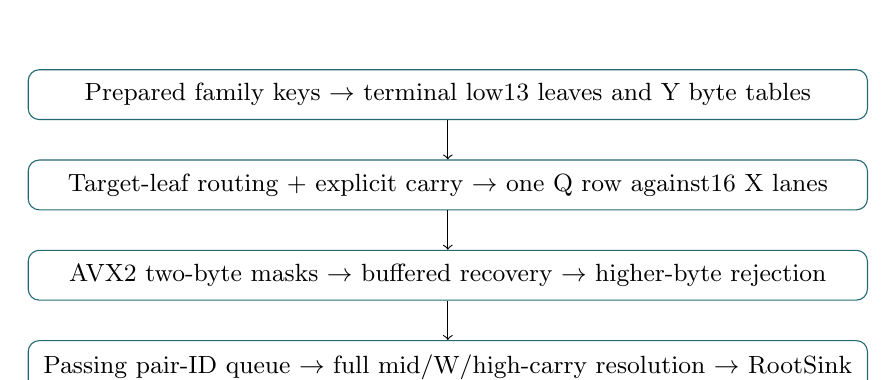
\begin{tikzpicture}[node distance=5mm,every node/.style={draw=teal,rounded corners,align=center,font=\small,text width=.85\linewidth,inner sep=5pt}]
\node (a) {Prepared family keys $\rightarrow$ terminal low13 leaves and Y byte tables};
\node (b) [below=of a] {Target-leaf routing + explicit carry $\rightarrow$ one Q row against16 X lanes};
\node (c) [below=of b] {AVX2 two-byte masks $\rightarrow$ buffered recovery $\rightarrow$ higher-byte rejection};
\node (d) [below=of c] {Passing pair-ID queue $\rightarrow$ full mid/W/high-carry resolution $\rightarrow$ RootSink};
\draw[->] (a)--(b);\draw[->] (b)--(c);\draw[->] (c)--(d);
\end{tikzpicture}
\end{center}


{\small\color{teal}Figure 1. Source-derived pipeline. The 16\ensuremath{\times}16 logical packet is evaluated as 16 row vectors, each containing 16 lanes. Only the first two bytes use the AVX2 table predicate; remaining checked bytes and full-key resolution occur afterward. Source:S6--S8; this is an architectural schematic, not a performance measurement.\par}

\subsection*{4.2. Routing and explicit carries}

For target leaf k and Q leaf i, choose j=(k-i-\ensuremath{\kappa}) mod 8192. The carry c=floor((i+j+\ensuremath{\kappa})/8192) is 0 or 1. In ascending Q-leaf order, carry-zero rows satisfy i\ensuremath{\leq}k-\ensuremath{\kappa} and carry-one rows form the remaining suffix. Offset lookup therefore splits processing into two contiguous ranges. The k=0,\ensuremath{\kappa}=1 edge has an empty carry-zero range and is handled through a signed split. [S8]


Write a=8192A+i and b=8192B+j. The corresponding mid sum is A+B+c, masked to m=min(32,W-13) bits. At n=108,m=32; at n=72,m=28. The first X block of each partner leaf is represented by one slot. An X leaf larger than sixteen contributes further blocks, with a correctly masked final block. The main row pass still visits Q rows whose partner X leaf is empty, but live mask zero prevents admission. Destinations with empty Y leaves are skipped entirely.


\subsection*{4.3. AVX2 predicate and masks}

For fixed Y\_k, the AVX2 path constructs lookup tables for byte 0 and byte 1. An unaligned 256-bit X load supplies sixteen 16-bit mid prefixes; the Q row is broadcast as a duplicated 32-bit word. \_mm256\_add\_epi16 computes sixteen independent low16 sums, with modular wrap. Since m\ensuremath{\geq}16 in this path, their two bytes are exactly the low two bytes of the full mid sum. Carry from the low byte into the high byte is naturally included. [S8]


The predicate uses byte shuffles to look up occupancy table bytes, chooses the appropriate 128-value half, selects each value's bit, and combines the two byte-failure bits per lane. If fail is the 32-byte failure mask and valid has bit 2\ensuremath{\ell} set for live lane \ensuremath{\ell}, then


\[
\mathrm{pass}=\mathord{\sim}\left(\mathrm{fail}\mathbin{|}(\mathrm{fail}\mathbin{\gg}1)\right)\mathbin{\&}\mathrm{valid}.
\]

Consequently, bit 2\ensuremath{\ell} survives only when both checked bytes occur in Y\_k's tables. The live mask excludes entries from the next leaf as well as final allocation padding. A 256-pair Cartesian packet is not processed in one SIMD instruction; it requires up to sixteen row evaluations.


\subsection*{4.4. Buffered recovery and materialization}

Each row writes a packed Q-position/pass-mask word to pending[n], then increments n only for nonzero masks. Survivor processing is outside this row loop. After a carry range is swept, the pending words are drained; set-bit positions recover the X-lane offset. The full masked 32-bit mid sum is recomputed, and checked chunks beyond the first two bytes are tested against Y occupancy tables. Passing lanes become explicit\{Q\_position, X\_position, carry\} records in a survivor queue. [S8]


The source-level main AVX2 row loop has fixed arithmetic and mask operations without a per-survivor call. This statement is local to that loop, not the overflow/resolver/control flow or a disassembly-derived claim about every compiled instruction. Only the first two bytes are vector-tested. Calling the entire four-byte predicate an all-SIMD filter would be inaccurate.


The queue is cleared for each target leaf but retains allocated capacity. Its initial reserve of 4096 is not a cap. Late materialization avoids an unconditional array of all source-pair sums, while still allowing many passing pair IDs to be stored. This distinction is essential to the memory model.


\subsection*{4.5. Exact resolver and scalar route}

For each queued pair, ARWLF recovers donor postings and scans every Y posting in that leaf. It compares the configured mid prefix, then the complete W-bit residual, then h high bits including residual carry. Only full prepared-key equality calls RootSink. Original stored quotient/residue and scalar structural checks follow where configured. Duplicate entries retain their distinct IDs and multiplicities. [S3,S6]


The scalar path traverses the same routed leaf geometry in packets no larger than 16\ensuremath{\times}16 and computes the same byte predicates from full mid sums. It is used when AVX2 is unavailable or fewer than two whole bytes are checked. A check\_bits=13 control forces a weaker scalar early filter while retaining full exact resolution; it is an instrumentation control, not a weaker final arithmetic contract.


\section*{5. Correctness and implementation limits}

\subsection*{5.1. Conditional routing invariant}

Proposition 1 (routing). For correctly prepared residual keys and \ensuremath{\kappa}\ensuremath{\in}\{0,1\}, every pair(a, b) maps to exactly one low13 target leaf, and its mid prefix equals(A+B+c) mod 2\textsuperscript{m} with the carry defined above.


Proof. Substitute a=8192A+i and b=8192B+j into a+b+\ensuremath{\kappa}. Euclidean division of i+j+\ensuremath{\kappa} by 8192 yields remainder k and quotient c. The remainder fixes j for given i, k,\ensuremath{\kappa}; the quotient enters the mid sum. Since i, j\ensuremath{\leq}8191 and \ensuremath{\kappa}\ensuremath{\leq}1, c is at most one. This is the identity implemented by both scalar routing and AVX2 carry ranges. Empty target leaves cannot contain a true match. First blocks plus overflow blocks partition each X leaf's entries, and live masks exclude only positions outside the block. \ensuremath{\square}


\subsection*{5.2. One-sided byte filtering}

Proposition 2 (necessary byte predicate). If a routed pair matches a Y entry on the checked mid prefix, every checked byte of its masked mid sum occurs in that leaf's corresponding byte table.


Proof. The tables are built by setting precisely those byte-value bits for every Y entry in the leaf. Equality of the checked prefix implies equality of each checked byte. The matched entry therefore supplies every required table bit. For a full-width28-bit prefix, masking zeros its unused top-byte bits in both stored mids and recomputed sums. Partial check modes test whole bytes conservatively; remaining exact comparisons follow. \ensuremath{\square}


These propositions justify no false negatives from routing and occupancy rejection under valid preparation. Their converse is false: several Y entries may jointly supply occupied bytes without any one matching the sum. The resolver removes those false positives.


\subsection*{5.3. Vector and exact-emission conditions}

Modulo 2\textsuperscript{1}\textsuperscript{6} addition preserves the low two bytes of the full mid sum. Combining both byte failures and valid bits implements the same two-byte condition as scalar evaluation. Higher-byte recomputation then applies the rest of the predicate. Final W-bit addition is safe because W\ensuremath{\leq}58, and the high-bit check includes the carry sum>>W. Thus every direct ARWLF emission satisfies the full prepared q\_bits-bit relation. Completeness applies to selected cells only when work\_divisor=1, execution is not aborted and resource operations succeed. Probe prefixes can return Completed for their requested partial scan; that status alone is not a completeness certificate. [S5,S6,S8]


The byte/lane equivalence is an algebraic argument about the intended predicate, supplemented by finite differential tests of its implementation. It is not inferred solely from a pass count. In particular, the test labelled scalar/AVX2 ``same lanes'' compares survivor counts, while final synthetic equality uses count and three commutative digest terms. Exact lane-ID streams are not directly compared in that assertion.


\subsection*{5.4. Correctness evidence and its boundaries}

A whole-value two-word modular oracle independently enumerates bounded synthetic roots at q\_bits=47 and 69, without leaf or carry decomposition. Cases include high-bit impostors, carry chains, duplicates, sparse and pooled dense leaves, overflow blocks and check widths 13,16,24/full. Scalar one-sided tests plant valid lanes over 20,000 rounds. Authentic n=72 tests compare upstream reporter results against frozen alternatives and shared downstream authority. [S10]


Fresh verification of the pinned snapshot passed all 55 Release CTest targets. The ARWLF executable reported 20,349 checks with zero failures. These are finite software checks, not 20,349 independent mathematical theorems. Historical 8/8 kernel and 10/10 campaign mutation claims are retained in prose but lack mutant definitions and execution transcripts; this audit does not promote them to independently reproduced results.


The large campaign's 221 completed cases all record their agreement gates as exact. Every case has zero full-key triples, residue-exact outputs, structural outputs and collected witnesses. Full-key equality/hash gates therefore also have empty-output coverage. Projected 25-bit hit counts are nonzero in 221/221 cases;32-bit counts in 204/221; mid-width counts in 123/221; and filter survivors in 137/221. These intermediate comparisons remain meaningful, while full-key and final witness equality are empty in every campaign case. Positive synthetic coverage and zero-output authentic agreement must be reported separately.


The benchmark API has narrower failure semantics than FullTer: ARWLF returns Completed, Aborted orNotApplicable, trusts prepared arrays, has no cancellation/resource ceiling and can allocate dynamically. RootSink's noexcept witness append can terminate on allocation failure. Snapshot 44-byte records at n=72 can be misaligned for uint64 pointer dereferences. Those source-audit issues were not demonstrated to corrupt the historical measurements, but passing x86 tests does not establish portable defined behavior. They require human review before production integration.


\section*{6. Complexity and cost model}

\subsection*{6.1. Logical pairs, lanes and rows}

For one selected cell let P\textsubscript{0}=|Q||X| and K be the occupied Y leaves. Actual valid routed lanes are


\[
V=\sum_{k\in K}\sum_i Q_iX_{(k-i-\kappa)\bmod8192}\leq P_0.
\]

The scalar packet census is


\[
P=\sum_{k\in K}\sum_{i:Q_iX_j>0}\left\lceil Q_i/16\right\rceil\left\lceil X_j/16\right\rceil,
\]

where j is the routed partner leaf. L=V/P. AVX2 row evaluations follow a different exact count:


\[
R=|Q||K|+\sum_{k\in K}\sum_{j:X_j>16}Q_{(k-\kappa-j)\bmod8192}\left(\left\lceil X_j/16\right\rceil-1\right).
\]

The first term includes zero-valid partner slots; the second counts overflow blocks. Logical P\textsubscript{0}, valid V, packets P and physical R are distinct. When every target leaf is populated, V=P\textsubscript{0}. On dense, roughly balanced leaves, vector width reduces the instruction cost per pair without changing its quadratic order on fixed hardware. No growing-word or distribution-independent subquadratic bound is established. [S6,S8,S9]


\subsection*{6.2. Setup, filtering and resolution}

Each touched family requires histogram/scatter and associated storage O(N\_family+8192). Fixed 8192-leaf table costs matter for small inputs. Let U count pairs passing the first two byte tests, including pairs rejected by later bytes; let S\_k be queued pairs surviving all byte predicates for target leaf k, S=\ensuremath{\Sigma}\_k S\_k, and E the emitted full-key triples. A source-faithful decomposition is


\[
T_{\mathrm{ARWLF}}\approx T_{\mathrm{build}}+\alpha R+\beta U+\gamma\sum_kS_kY_k+T_{\mathrm{emit+authority}}(E).
\]

Here \ensuremath{\alpha},\ensuremath{\beta},\ensuremath{\gamma} are hardware/input-dependent coefficients, not fitted constants in this study. The first term covers local packing and target tables, the next terms separate vector filtering, two-byte-passing lane recovery/higher-byte testing and the explicit all-Y-in-leaf resolver. Queue insertion depends on S, a subset of U; a separate S term can be retained when fitting a future model. A low-selectivity adversarial leaf can admit all pairs and compare them to every target entry, yielding cubic comparison work. The favorable experiment is therefore a finite regime, not a worst-case theorem.


For K2 a useful decomposition is T\_K2\ensuremath{\approx}T\_tile(P\textsubscript{0})+T\_bitmap(H\_coarse)+T\_group(H\_19)+T\_authority(H\_expanded). K2\_WIDE adds wider comparisons before authority. Projected survivors and expanded ID triples need not have the same cardinality because a projected key can have multiple postings. A simplified c\_KP\textsubscript{0}+c\_SH\_low is an explanatory approximation only after defining H\_low; it must not silently equate bitmap hits, pairs and output triples.


\subsection*{6.3. Memory bound}

ARWLF stores linear input/posting structures and per-family fixed leaf tables, plus pending row scratch and a dynamically growing pair-ID queue. Its auxiliary bound is


\[
O\!\left(N_{\mathrm{touched}}+8192f_{\mathrm{touched}}+\max_s|Q_s|+\max_{\mathrm{cell},k}S_k\right).
\]

with optional emitted witness storage and allocation capacities in addition. A single all-pass leaf permits S\_k=\ensuremath{\Theta}(|Q||X|). Consequently the architecture document's unconditional ``pairless O(N)'' wording is too strong for the implemented code. The defensible statement is that ARWLF avoids unconditional complete pair-sum materialization, while storage depends on passing pairs for the current target leaf. Neither reported index\_bytes nor initial reserve proves a process peak-memory ceiling. [S6,S11]


\section*{7. Adaptive backend selection}

\subsection*{7.1. Candidate rules and prediction}

The frozen dispatcher considers QUEUE\_DENSE when distinct-family group capacities permit it, K2\_WIDE when full keys exist, and ARWLF when its width domain and packet-density criterion permit it. Its ARWLF criterion computes all-Q/X packet geometry irrespective of occupied Y destinations, so it is not identically the routed census L\ensuremath{\geq}16 for arbitrary inputs. In the evaluated dense-Y thinning family it acts approximately as that conservative threshold. [S12]


It chooses a deterministic probe from at most the first eight encountered Q and X families. Nominal probe budgets are 2\textsuperscript{2}\textsuperscript{1} pairs for K2\_WIDE and 2\textsuperscript{2}\textsuperscript{6} for ARWLF, with power-of-two work divisors and ceiling rounding. K2\_WIDE extrapolates by scanned pair mass. ARWLF separately scales measured construction by touched entries and measured processing by modeled main rows. QUEUE\_DENSE uses minima from two build-only and two total probes, then scales processing by pair mass. These models omit explicit survivor/resolver and overflow terms.


Stable ties favor QUEUE\_DENSE, ARWLF, K2\_WIDE. The source comment saying K2\_WIDE wins ties disagrees with that actual order. An ARWLF winner receives one prefix guard comparing observed modeled cost to runner-up prediction after enough target leaves and at least 65536 modeled pairs. A header still says 2\textsuperscript{2}\textsuperscript{0}; code uses 2\textsuperscript{1}\textsuperscript{6}. Aborted output is discarded by resetting the sink before a complete runner-up invocation. This is a timing heuristic, not a mathematical regret bound. Probe costs are included in measured dispatch time.


\subsection*{7.2. Measured regime behavior}

On all 29 authentic n=108 microproblems, dispatch executes ARWLF and chooses the fastest measured backend. Its median regret is 1.0101 and maximum 1.0258. On four n=72 whole-root replays, it selects QUEUE\_DENSE, with median regret 1.0584 and maximum 1.1403. These favorable results coexist with substantial overhead: on 68 n=72 microproblems, median regret is 87.17 and maximum 172.87, with backend work around 0.07--0.17 ms versus dispatch around 8--14 ms. Near-equal fastest-backend labels at this scale are noise-sensitive, but probe overhead itself is unambiguous.


Source-thinned n=108 cases have median regret 2.193 and maximum 17.639. ARWLF wins controlled comparisons around L=2, yet the frozen applicability guard excludes it below roughly 16; observed L at requested 16 can sit just below the boundary. The paper reports this evaluated behavior without retroactively tuning thresholds.


\section*{8. Experimental methodology}

\subsection*{8.1. Revision and execution provenance}

The connected GitHub main branch was resolved before analysis to commit 8e9fe7fdda447088738b5e682ba6aea4cf83a121, dated 2 October 2026 at 16:24:09UTC, tree fd469e34cb62e7342bc4b38a76c13e668a8e7f06. All 214 tracked blobs were checked against the local archive, accounting for Git's CRLF export conversion. This is a private-source study; external readers currently need authorized artifact access. No source modifications or expensive benchmark campaign were performed during the audit. Fresh tests ran from an immutable archive into external build directories.


Historical campaign metadata identifies an Intel Core Ultra 9 275HX, single-thread execution pinned to logical P-core23, EcoQoS disabled, AC checks at process boundaries, Release MSVC 195136257 and TER\_NATIVE\_OPT=ON. Recorded flags enable AVX2 globally. Default non-native builds isolate specialized AVX2 translation units and omit frozen-library IPO, but the evaluated native build cannot be described as universally ISA-confined. ARWLF additionally checks CPUID/OSXSAVE/XCR0; donor K2 selection relies on caller gating. The campaign executable refuses an unavailable AVX2 runtime. [S13]


No committed thermal, frequency, contention, package-power or memory-frequency traces establish a constant machine state. AC checks are sampled, not continuous. Snapshot loading, generic target preparation, full family keys, root index, census, thinning calibration and correctness passes are outside each backend timing. ARWLF's local cache construction and dispatch probes are inside. Sorting/comparing collected residue-ID witnesses follows the timer, while candidate authority and witness-vector writes remain inside.


\subsection*{8.2. Workload families and sample units}

The regime archive contains 224 case identities:101 completed AUTHENTIC\_FULLTER cases,111 completed AUTHENTIC\_SOURCE\_THINNED cases, nine completed AUTHENTIC\_TARGET\_THINNED cases and three unreachable source-thinning requests. Among authentic cases,29 are n=108 microproblems and 72 are n=72 measurements (four whole roots and 68 microproblems). No whole n=108 root replay or complete-solver timing is present.


The capture path requests FullTer complete lists under finite parameters. Its original coefficients are n-bit random values, while the original target is overwritten by the sum of a deterministic planted subset. TER Random target mode concerns internal decomposition targets. This data origin must accompany ``authentic'': it identifies complete captured TER lists rather than an independently random original target distribution. Classic-capture comparison is recorded for n=72 snapshots, not the six n=108 snapshots. The large snapshot files themselves are absent; retained hashes/censuses and source describe their identities and origin, not independently repeated capture in this audit.


The anchor cell 2730 is fixed by a deterministic shuffle. Stratified discovery uses a 4\ensuremath{\times}4 quartile grid on log\textsubscript{2} pair mass and L. An amendment selects n=108 corner strata after census and before timing; n=72 retains all strata. We reconstructed all ten roots' selected cells from integer census fields. Calibration has 14 selected n=108 cases from roots 0x1001,0x2003,0x3007; holdout has 15 from 0x4001,0x5003,0x6007. ``Holdout'' is the recorded campaign role, not proof that every historical tuning decision was uninfluenced by those roots.


\subsection*{8.3. Protocol and statistical recomputation}

The 221 completed cases mix 201 discovery cases with one warmup and three timed rounds, and 20 final cases with three warmups and seven timed rounds. Backend order rotates by absolute round and reverses on odd rounds. It is deterministic interleaving rather than randomized scheduling. Final protocols cover whole roots, anchors and crossover confirmations; selected corner strata remain discovery measurements.


Per-case speedup is the ratio of backend medians. Group summaries are equal-case geometric means, with 10000-draw percentile bootstraps at seed 0xB007. We independently recomputed medians, quartiles, ranges, speedups, regret and both case and root-cluster confidence intervals. To match exact printed endpoints we reproduced the original sequential RNG consumption; independently reset RNG calculations are also retained. The three roots per split are the more relevant independence unit than 14 or 15 correlated cells. These intervals express conditional resampling uncertainty, not universal population coverage.


The raw sample file contains 3229 rows. Matching root, case, backend and completed process-attempt identity accepts 3220; nine rows from a partial invocation remain explicitly preserved. Pooling them by case alone changes three backend medians in one source-thinning case. With correct process reconciliation, all committed medians/quartiles/extrema and both plotting tables reproduce within printed rounding. Headline authentic results are unaffected. [S14]


\subsection*{8.4. Exactness and measurement stability}

Untimed gates compare full-key counts/digests, k 32 projected counts, intermediate width counts, downstream authority, sorted residue-ID lists, clean directory state and independent census. Every timed and warmup sample rechecks the final digest and sorted witness vector outside elapsed time. The eight recorded gate fields pass on 221 completed cases. All full-key counts and downstream exact/structural/witness vectors are empty, so large-instance positive-witness correctness remains unestablished by this campaign alone.


The fixed-work CPU sentinel has 124 observations, min 65.396 ms, median 66.692 ms and max 92.307 ms, a 41.15\% min-to-max spread. Completed initial n=72 process end readings reach 74.10--80.55 ms. This contradicts result prose restricting elevated values to resume starts or source-thinning phases. Many n=108 corner, Y-ablation and confirmation readings lie near 65--67 ms, but matched ratios do not prove that state effects cancel equally across algorithms. An earlier separate v 3 run on root0x3007 records roughly 79.8\ensuremath{\times} versus K2; the regime anchor gives 52.75\ensuremath{\times}. Both remain preserved, with the preregistered regime as the primary result and the discrepancy unexplained by direct machine-state traces.


\section*{9. Results}

\subsection*{9.1. Dense n=108 microproblems}

{\small\setlength{\tabcolsep}{3pt}\begin{longtable}{p{0.174\linewidth} p{0.174\linewidth} p{0.174\linewidth} p{0.174\linewidth} p{0.174\linewidth}}
\toprule

\textbf{Set} & \textbf{Cases / source roots} & \textbf{ARWLF speedup over K2: geometric mean} & \textbf{Case-bootstrap95\% interval} & \textbf{Root-bootstrap95\% interval} \\
\midrule\endhead

Calibration & 14 /3 & 53.0875\ensuremath{\times} & 50.2883--57.0716\ensuremath{\times} & 48.1746--57.6058\ensuremath{\times} \\

Holdout & 15 /3 & 52.8933\ensuremath{\times} & 51.1931--55.0112\ensuremath{\times} & 51.8107--53.8149\ensuremath{\times} \\

\bottomrule\end{longtable}}

{\small\color{teal}Table 2. Ratios median(K2)/median(ARWLF), equal-case geometric means from accepted raw samples. Source:results/arwlf/regime-20261001/samples.csv, cases.csv and census; independent analysis/benchmark\_statistics.json. Timing unit is milliseconds before division; ratios and intervals are dimensionless. Case and root resampling use10000 draws.\par}

Calibration speedups range 46.49--78.10\ensuremath{\times} and holdout 46.91--63.20\ensuremath{\times}. K2\_WIDE is 29.57--33.35\ensuremath{\times} slower than ARWLF across the same 29 selected microproblems, with median 32.74\ensuremath{\times}. Similar calibration/holdout means strengthen the finite result within these captured roots, while the small number of roots limits distributional inference. Generic preparation is excluded and no scaling from these microproblems to a full n=108 root is measured.



\begin{center}
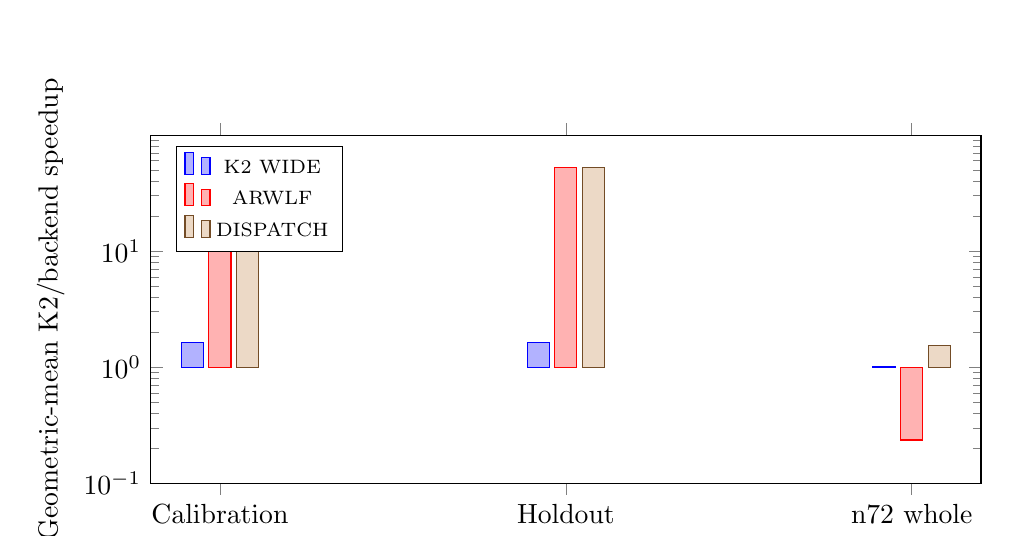
\begin{tikzpicture}\begin{axis}[ybar,ymode=log,width=\linewidth,height=6cm,ylabel={Geometric-mean K2/backend speedup},symbolic x coords={Calibration,Holdout,n72 whole},xtick=data,legend style={font=\scriptsize},legend pos=north west,bar width=8pt,ymin=.1]
\addplot coordinates {(Calibration,1.6196641) (Holdout,1.6306085) (n72 whole,1.0083157)};\addlegendentry{K2 WIDE}
\addplot coordinates {(Calibration,53.087514) (Holdout,52.893324) (n72 whole,0.23540226)};\addlegendentry{ARWLF}
\addplot coordinates {(Calibration,52.364881) (Holdout,52.381929) (n72 whole,1.5350592)};\addlegendentry{DISPATCH}
\end{axis}\end{tikzpicture}
\end{center}


{\small\color{teal}Figure 2. Geometric means of per-case speedups against K2:14 calibration and 15 holdout n=108 microproblems versus four n=72 whole-root replays. Source:accepted raw regime samples and case metadata. Whole roots and microproblems are separate measurement units; the bars do not estimate full-solver throughput.\par}

\subsection*{9.2. Sparse whole roots and controlled crossover}

For four n=72 whole-root replays, K2 medians are 301.5,327.7,545.3 and 551.5 ms; QUEUE\_DENSE gives 167.6,269.9,298.1 and 299.2 ms. ARWLF is slower than K2, with speedup approximately 0.14--0.30\ensuremath{\times}. These negative results are compatible with its fixed leaf-table/setup and row-scan costs overwhelming sparse work. QUEUE\_DENSE is an important complement, not a defeated universal baseline.


Source thinning spans 105 discovery cases and six final confirmations over three calibration n=108 roots. Three L=96 requests on 0x1001 are unreachable and remain recorded. Discovery geometric means cross between observed L\ensuremath{\approx}1 and L\ensuremath{\approx}2; final L\ensuremath{\approx}2 comparisons give about 3.44\ensuremath{\times},2.73\ensuremath{\times} and 2.74\ensuremath{\times} ARWLF speedup over K2\_WIDE, while L\ensuremath{\approx}1 loses. Final confirmations retain the deterministic discovery geometry for their matching seed. The bracket describes this thinning family; pair mass changes substantially and the smallest workloads are dominated by overhead.



\begin{center}
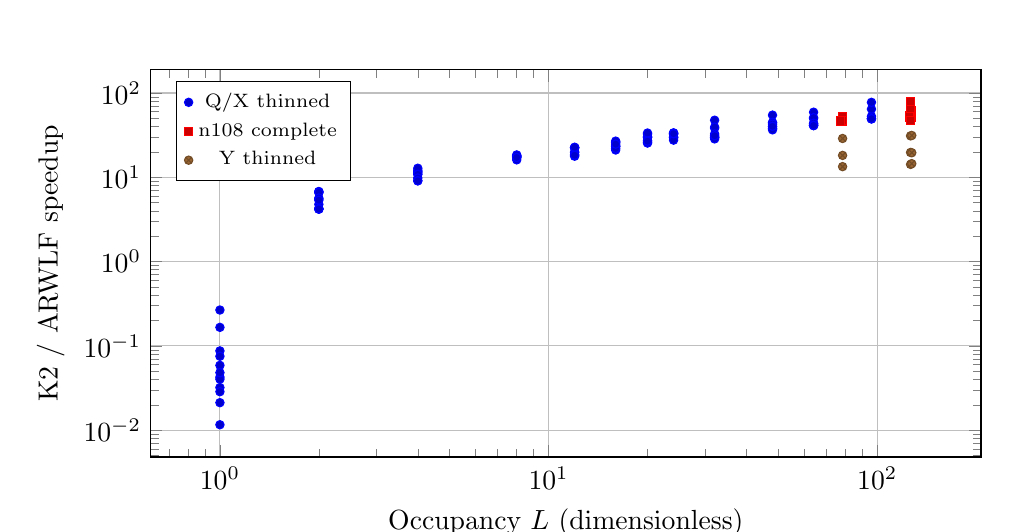
\begin{tikzpicture}\begin{loglogaxis}[width=\linewidth,height=6.5cm,xlabel={Occupancy $L$ (dimensionless)},ylabel={K2 / ARWLF speedup},legend style={font=\scriptsize},legend pos=north west,grid=major]
\addplot+[only marks,mark size=1.5pt] coordinates {(1,0.08734377) (1,0.04267617) (1,0.1660502) (1.9998,6.778957) (1.9996,6.742323) (1.9997,6.608846) (4,11.49112) (4,12.12048) (3.9998,11.6839) (7.9998,17.89837) (7.9996,18.0169) (7.9998,17.73705) (11.9998,22.43912) (11.9997,22.25695) (11.9997,22.50183) (15.9998,26.04472) (15.9997,25.99204) (15.9998,21.06754) (19.9993,29.60296) (19.9997,29.88751) (19.9996,30.25769) (23.9995,30.12466) (23.9998,33.62511) (23.9997,33.45222) (31.9998,38.31122) (31.9993,47.50335) (31.9996,39.34858) (47.9997,54.57959) (47.9997,44.25684) (47.9997,44.76242) (63.9998,59.12802) (63.9996,49.72265) (63.9994,50.94098) (1,0.07539332) (1,0.03209933) (1,0.02865361) (1.9999,6.605752) (1.9998,5.526031) (1.9998,5.665452) (3.9997,10.92202) (4,12.80436) (4,10.84666) (7.9997,17.68274) (7.9999,16.97212) (7.9998,16.09164) (11.9999,19.7233) (11.9999,19.93347) (11.9996,18.54994) (15.9999,23.16309) (15.9999,23.28469) (16,23.5662) (19.9995,25.75806) (19.9999,32.58554) (19.9996,25.48043) (23.9997,32.48895) (23.9995,29.37189) (23.9995,29.5154) (31.9994,29.90361) (32,29.68223) (31.9994,29.88113) (47.9994,38.25594) (47.9999,42.69084) (47.9993,37.75655) (64,42.78838) (64,42.8956) (63.9997,43.78171) (95.9992,52.92674) (95.9993,64.42228) (95.9993,77.41283) (1,0.02123914) (1,0.2666064) (1,0.05886345) (1.9999,4.190963) (2,4.775927) (1.9998,4.199954) (3.9997,9.799617) (3.9999,9.094852) (3.9998,9.067909) (8,17.32317) (7.9997,18.41758) (7.9998,17.20578) (11.9997,22.68564) (11.9996,17.77812) (11.9996,18.25612) (15.9995,22.00255) (15.9998,26.83669) (15.9998,24.74743) (19.9996,27.30205) (19.9995,33.48263) (19.9997,26.80723) (23.9998,32.71999) (23.9995,27.57082) (23.9999,32.88371) (31.9996,32.65197) (31.9997,28.53132) (31.9997,31.10904) (47.9995,40.13695) (47.9996,36.53581) (47.9999,40.19698) (63.9991,41.03017) (63.9997,41.08702) (63.9999,41.1704) (95.9996,49.56516) (95.9994,49.18909) (95.9995,49.4213) (1,0.04034801) (1.9998,5.347406) (1,0.04818936) (1.9999,4.266508) (1,0.01161977) (1.9999,4.211326)};\addlegendentry{Q/X thinned}
\addplot+[only marks,mark size=1.5pt] coordinates {(78.4361,52.89416) (126.2576,78.09815) (127.3255,52.75364) (125.9366,50.66372) (126.1318,51.75914) (125.5637,52.41031) (78.3667,46.70708) (78.1783,46.89279) (77.3929,46.49186) (125.5627,53.14348) (126.7159,53.98476) (126.6461,53.25356) (125.7078,53.16424) (126.5336,52.90131) (125.5588,53.06494) (125.5379,52.55476) (126.5963,53.10692) (125.4932,51.70407) (126.5404,52.15036) (125.5276,52.32923) (126.5007,52.22428) (125.5147,51.91003) (126.5527,52.19955) (125.5716,51.85948) (126.4813,62.05554) (126.1819,63.20225) (125.0904,51.93079) (125.0842,52.18731) (126.179,46.90986)};\addlegendentry{n108 complete}
\addplot+[only marks,mark size=1.5pt] coordinates {(78.4362,28.85646) (78.4361,18.17663) (78.436,13.3752) (126.2576,30.98387) (126.2572,19.70831) (126.258,14.21658) (127.3254,31.3372) (127.3255,19.54672) (127.3255,14.50725)};\addlegendentry{Y thinned}
\end{loglogaxis}\end{tikzpicture}
\end{center}


{\small\color{teal}Figure 3. Per-case median(K2)/median(ARWLF) versus routed lane occupancy L. Source:accepted raw regime samples and committed census/case geometry. Points distinguish 29 complete-list n=108 microproblems,111 source-thinned cases and nine Y-thinned cases; ratios and L are dimensionless. Protocols include discovery and final repetitions. No fitted asymptotic curve is implied.\par}

\subsection*{9.3. Dispatcher behavior}

{\small\setlength{\tabcolsep}{3pt}\begin{longtable}{p{0.174\linewidth} p{0.174\linewidth} p{0.174\linewidth} p{0.174\linewidth} p{0.174\linewidth}}
\toprule

\textbf{Regime} & \textbf{Cases} & \textbf{Median regret} & \textbf{Maximum regret} & \textbf{Fastest measured backend selected} \\
\midrule\endhead

n=108 authentic microproblems & 29 & 1.0101 & 1.0258 & 29/29 \\

n=72 whole roots & 4 & 1.0584 & 1.1403 & 4/4 \\

n=72 microproblems & 68 & 87.17 & 172.87 & 6/68 \\

n=108 source-thinned & 111 & 2.193 & 17.639 & 63/111 \\

n=108 Y-thinned & 9 & 1.0093 & 1.0199 & 9/9 \\

\bottomrule\end{longtable}}

{\small\color{teal}Table 3. Regret is median(dispatch)/minimum legal-backend median, including probe costs. Source:accepted raw regime samples; independent dispatcher statistics. Near-tied choices in tiny cases are sensitive to timing noise. Mixing these units into one global regret headline would hide the dominant overhead failure.\par}


\begin{center}
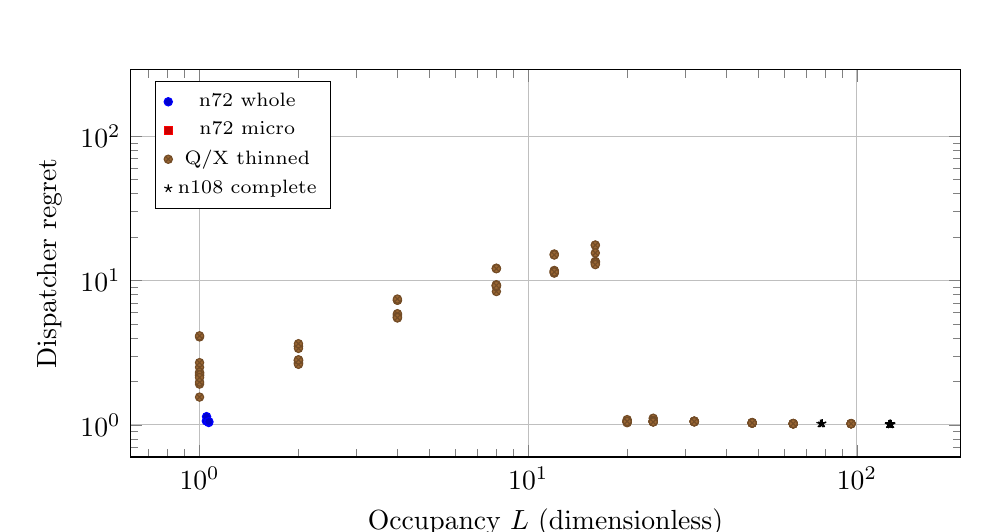
\begin{tikzpicture}\begin{loglogaxis}[width=\linewidth,height=6.5cm,xlabel={Occupancy $L$ (dimensionless)},ylabel={Dispatcher regret},legend style={font=\scriptsize},legend pos=north west,grid=major]
\addplot+[only marks,mark size=1.5pt] coordinates {(1.0488,1.063388) (1.0504,1.140317) (1.0665,1.038629) (1.0673,1.053506)};\addlegendentry{n72 whole}
\addplot+[only marks,mark size=1.5pt] coordinates {(1.0558,172.8713) (1.0359,147.3935) (1.0444,104.8321) (1.0627,150.8403) (1.0447,160.4913) (1.0617,113.5056) (1.0513,152.9747) (1.0512,147.7902) (1.0517,121.9328) (1.0628,162.8515) (1.0521,146.6852) (1.0353,137.5418) (1.0444,163.6306) (1.0448,113.8568) (1.0361,112.7152) (1.0622,130.5448) (1.0357,113.2288) (1.0618,119.3552) (1.0539,122.6763) (1.0633,139.2973) (1.0462,138.7397) (1.0377,116.1703) (1.0629,115.0057) (1.0363,108.2139) (1.0538,125.0603) (1.0644,110.226) (1.0538,128.4581) (1.0463,117.12) (1.0656,99.35565) (1.0467,111.5416) (1.0463,92.98619) (1.0547,106.8414) (1.0374,113.9632) (1.0384,103.3169) (1.0721,75.47714) (1.0702,76.52387) (1.0799,74.51469) (1.0534,63.92562) (1.0527,76.58942) (1.0621,71.23213) (1.0621,78.61606) (1.0698,69.84751) (1.0697,80.79665) (1.0615,67.14517) (1.0539,70.49689) (1.0811,78.60313) (1.0814,72.22151) (1.0514,77.82187) (1.0815,81.34886) (1.0704,73.0393) (1.0616,74.8951) (1.0713,67.67871) (1.0698,73.15673) (1.0806,73.35747) (1.0708,75.73904) (1.0787,76.46979) (1.063,70.21319) (1.07,72.0696) (1.0708,66.79803) (1.0809,66.24052) (1.0541,70.72618) (1.0546,72.79945) (1.0541,72.48615) (1.0542,65.53065) (1.0629,77.67755) (1.0633,71.16041) (1.0635,65.62491) (1.0824,67.94444)};\addlegendentry{n72 micro}
\addplot+[only marks,mark size=1.5pt] coordinates {(1,2.283784) (1,1.916667) (1,1.98057) (1.9998,3.50344) (1.9996,3.510115) (1.9997,3.388717) (4,7.310235) (4,7.309037) (3.9998,7.453541) (7.9998,12.13961) (7.9996,12.18027) (7.9998,12.085) (11.9998,15.29562) (11.9997,15.07215) (11.9997,15.06634) (15.9998,17.6387) (15.9997,17.58848) (15.9998,15.54039) (19.9993,1.05812) (19.9997,1.058636) (19.9996,1.064072) (23.9995,1.112253) (23.9998,1.064577) (23.9997,1.063403) (31.9998,1.054621) (31.9993,1.06338) (31.9996,1.060356) (47.9997,1.038963) (47.9997,1.028616) (47.9997,1.034634) (63.9998,1.020078) (63.9996,1.015422) (63.9994,1.017586) (1,2.193457) (1,2.509804) (1,2.70082) (1.9999,2.667106) (1.9998,2.792685) (1.9998,2.782701) (3.9997,5.816107) (4,5.701115) (4,5.896773) (7.9997,9.221784) (7.9999,9.36194) (7.9998,9.253929) (11.9999,11.66304) (11.9999,11.75617) (11.9996,11.27059) (15.9999,13.58274) (15.9999,13.44519) (16,13.48302) (19.9995,1.045621) (19.9999,1.087747) (19.9996,1.0484) (23.9997,1.053915) (23.9995,1.052352) (23.9995,1.055266) (31.9994,1.052664) (32,1.048218) (31.9994,1.057686) (47.9994,1.031058) (47.9999,1.031036) (47.9993,1.027365) (64,1.019261) (64,1.018549) (63.9997,1.023309) (95.9992,1.019119) (95.9993,1.020381) (95.9993,1.017428) (1,4.069767) (1,1.558171) (1,2.317121) (1.9999,2.667909) (2,2.710769) (1.9998,2.627738) (3.9997,5.595795) (3.9999,5.508842) (3.9998,5.532836) (8,8.396201) (7.9997,9.082276) (7.9998,9.253205) (11.9997,11.50749) (11.9996,11.32696) (11.9996,11.47696) (15.9995,13.23647) (15.9998,13.27138) (15.9998,12.90416) (19.9996,1.034643) (19.9995,1.05376) (19.9997,1.057169) (23.9998,1.052196) (23.9995,1.052935) (23.9999,1.046539) (31.9996,1.054965) (31.9997,1.057801) (31.9997,1.052322) (47.9995,1.029156) (47.9996,1.03323) (47.9999,1.031972) (63.9991,1.016827) (63.9997,1.01593) (63.9999,1.020437) (95.9996,1.020234) (95.9994,1.019674) (95.9995,1.018148) (1,2.220253) (1.9998,3.652975) (1,2.127036) (1.9999,2.815784) (1,4.142857) (1.9999,2.82331)};\addlegendentry{Q/X thinned}
\addplot+[only marks,mark size=1.5pt] coordinates {(78.4361,1.025825) (126.2576,1.013282) (127.3255,1.009837) (125.9366,1.009717) (126.1318,1.010104) (125.5637,1.009476) (78.3667,1.020336) (78.1783,1.019238) (77.3929,1.019079) (125.5627,1.010801) (126.7159,1.00972) (126.6461,1.002201) (125.7078,1.009716) (126.5336,1.009998) (125.5588,1.011651) (125.5379,1.012637) (126.5963,1.01912) (125.4932,1.007894) (126.5404,1.012262) (125.5276,1.009721) (126.5007,1.009003) (125.5147,1.010813) (126.5527,1.00712) (125.5716,1.01083) (126.4813,1.013535) (126.1819,1.007461) (125.0904,1.008522) (125.0842,1.008358) (126.179,1.01165)};\addlegendentry{n108 complete}
\end{loglogaxis}\end{tikzpicture}
\end{center}


{\small\color{teal}Figure 4. Per-case dispatcher regret against L, with n=72 microproblems, n=72 whole roots, n=108 authentic microproblems and source-thinned n=108 cases marked separately. Source:accepted raw timings and case geometry;68+4+29+111 cases. Both axes are dimensionless. The plot records the frozen selection behavior, including applicability and probe overhead weaknesses.\par}

\subsection*{9.4. Target-density ablation}

Nine cases retain 1/2,1/4 or 1/8 of Y for each calibration n=108 anchor, with fixed Q/X. K2/ARWLF speedup ranges fall from 28.86--31.34\ensuremath{\times} at half Y to 18.18--19.71\ensuremath{\times} at quarter Y and 13.38--14.51\ensuremath{\times} at eighth Y. K2\_WIDE/ARWLF ratios similarly fall from 20.27--20.91\ensuremath{\times} to 10.30--10.66\ensuremath{\times}. ARWLF remains faster, while the gap shrinks substantially as target density decreases.



\begin{center}
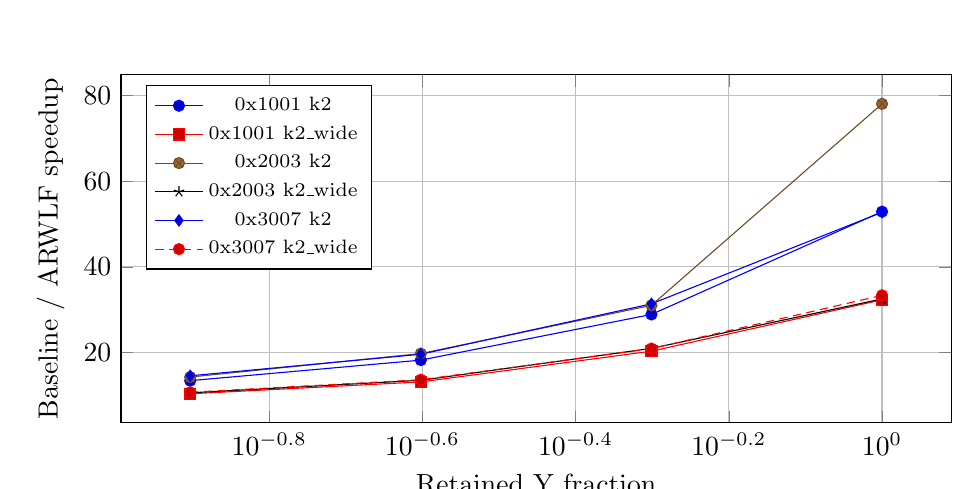
\begin{tikzpicture}\begin{semilogxaxis}[width=\linewidth,height=6cm,xlabel={Retained Y fraction},ylabel={Baseline / ARWLF speedup},legend style={font=\scriptsize},legend pos=north west,grid=major]
\addplot+ coordinates {(0.125,13.375197) (0.25,18.176626) (0.5,28.856458) (1,52.894163)};\addlegendentry{0x1001 k2}
\addplot+ coordinates {(0.125,10.301418) (0.25,13.078826) (0.5,20.267639) (1,32.280304)};\addlegendentry{0x1001 k2\_wide}
\addplot+ coordinates {(0.125,14.216576) (0.25,19.708307) (0.5,30.98387) (1,78.098154)};\addlegendentry{0x2003 k2}
\addplot+ coordinates {(0.125,10.526695) (0.25,13.463254) (0.5,20.913689) (1,32.49346)};\addlegendentry{0x2003 k2\_wide}
\addplot+ coordinates {(0.125,14.507254) (0.25,19.546722) (0.5,31.337203) (1,52.753641)};\addlegendentry{0x3007 k2}
\addplot+ coordinates {(0.125,10.656639) (0.25,13.58715) (0.5,20.876967) (1,33.328704)};\addlegendentry{0x3007 k2\_wide}
\end{semilogxaxis}\end{tikzpicture}
\end{center}


{\small\color{teal}Figure 5. Median baseline/ARWLF ratios at all-Y anchors and controlled Y-retention fractions. Source:accepted raw timings for three calibration anchors and nine target-thinned cases. Q/X are held fixed; each root has one Y-thinning seed. All-Y anchors use the final protocol, while thinned cases use discovery repetitions. Ratios and retained fraction are dimensionless.\par}

\section*{10. Mechanistic interpretation}

The source exposes two changes. ARWLF replaces a tile/gather projected filter with target-leaf16-bit row arithmetic and byte-table masks. It also keeps pair identities implicit until stronger byte rejection, then applies full residual and high-bit checks before shared authority. The comparison with K2\_WIDE matters: both reach the same full-key relation, but one retains the narrow K2 front end and its scalar group processing. The large remaining gap is consistent with pair-processing and materialization costs beyond authority calls alone.


The Y ablation supplies a second, partial control. At fixed source lists, lower target density reduces opportunities for projected matches, group expansion and survivor work. K2 runtime falls much more than ARWLF runtime, so projected-survivor traffic plausibly contributes to K2's dense-target cost. ARWLF does change with Y; ``barely changes'' would overstate invariance. Lower Y also changes occupied leaves, byte tables and resolver comparisons, so this experiment does not uniquely isolate one mechanism or assign percentages of speedup.


The cost model predicts complementary regimes. When substantial source-pair traffic is well packed and target-byte predicates are selective, cheap row scanning plus sparse recovery can dominate. When source work is tiny, fixed tables and probes dominate; when distinct residual occupancy permits cheap word intersections, QUEUE\_DENSE can win. In adversarial saturated byte tables, pair recovery and all-Y-leaf comparisons can dominate. These are source-derived expectations consistent with the measurements, not an empirically fitted universal performance law.


\section*{11. Related work and novelty boundary}

Baran, Demaine and Pătraşcu use packed approximate additive filtering with subsequent exact verification in subquadratic3SUM algorithms [1]. Their pseudolinear hashing and word-RAM packing are closer conceptual antecedents than a generic appeal to SIMD. The randomized asymptotic model differs from deterministic fixed-width TER replay. Chen, Jin, Randolph and Servedio's Subset Sum algorithm likewise combines bit packing, approximate additive conditions and full checking [2]. ARWLF claims neither their polynomial improvement nor priority for packed additive filtering.


Li supplies the TER construction and signed-representation context [3]. The present repository implements finite complete-list semantics and tests modular arithmetic; its reporter measurements do not establish the paper's heuristic asymptotic success assumptions or a new exponent. Practical parallel two-list Subset Sum predates this work, including Wan et al.'s GPU implementation [4]; different workload/processor scopes preclude a quantitative comparison with these CPU replay timings.


Late materialization is established in column-oriented execution [5], and radix/cache organization and hardware-sensitive join tuning are established systems practices [6]. SIMD selection and partitioning also have substantial prior database work [7]. ARWLF's contribution is therefore its specific composition for TER: terminal target-leaf routing with exact carries, row predicates, deferred ID recovery and measured regime characterization. SIMD, radix, packing, carry-aware arithmetic, meet-in-the-middle, late materialization and adaptive selection are conceded ingredients. No first-use claim is supported by the current literature search.


\section*{12. Limitations and research implications}

The evaluated implementation remains a benchmark root reporter. It does not integrate canonical parent materialization, deduplication, solver attempt control or production resource semantics. Its worst-case passing-pair storage can be quadratic and resolver comparisons cubic. The 53\ensuremath{\times} result concerns selected n=108 microproblems after generic preparation, not full-root or full-solver runtime. No n=144 measurement is committed.


The hardware result is single-machine, AVX2-specific and native-build-dependent. Three source roots per calibration/holdout split, deterministic cells and correlated shared lists limit independent statistical support. Original targets are planted. All campaign final witnesses are zero. Ten raw snapshots and the original executable are absent, so byte-identical input/binary replay was not performed. Historical mutation counts are documentation-supported rather than independently reproduced. Sentinel drift and prior-v3 variation prevent a claim of fully controlled machine state.


Before production use, the replay APIs require explicit input/resource/abort contracts, safe snapshot loads, bounded or accounted survivor/witness allocation and stronger forced dispatcher fallback coverage. Before publication, a positive-output authentic campaign, original snapshot release or verified regeneration, more independent roots/machines and isolated mechanism measurements would strengthen the study. None was silently added here. The finite engineering result is worth reporting with these boundaries; it does not resolve the earlier output-sensitive Stage-D research objective.


\section*{13. Reproducibility and artifact availability}

The audit package records the connected revision/tree, all 214 file classifications, source evidence, independent analysis scripts, raw-statistical reconciliation, figure/table provenance, build logs and a human-review checklist. The campaign's current freeze manifest protects 29 source files after CR removal. All 29 match the historical campaign source closure under line-ending normalization. Of 137 historical manifest entries,119 match, six cached Python files are absent and twelve supporting source/script/config entries differ. Thus the narrow frozen-closure claim holds; an unchanged-entire-tree claim does not.


The ten input hashes, list sizes and capture commands are committed, while snapshot bytes are not. Reproduction requires recovering the historical files with matching SHA256, or recapturing and comparing logical record identities under the recorded source/environment. Capture elapsed time and process-memory fields enter the serialized header/checksum, so logical determinism does not guarantee the same whole-file hash. Fresh Release tests used MSVC 19.51.36257.0 with TER\_NATIVE\_OPT=OFF in a build directory outside the source. They validate the pinned source's registered tests, not historical performance. The accompanying appendix separates commands actually executed from expensive campaigns that were only inspected. The private repository and manuscript author/affiliation/availability metadata require human completion before submission.


\section*{14. Conclusion}

On the evaluated complete-list n=108 TER root microproblems, ARWLF delivers independently recomputed 53.09\ensuremath{\times} calibration and 52.89\ensuremath{\times} holdout speedups over K2. The implementation makes dense pair filtering cheaper and defers scalar ID materialization until stronger target-derived rejection. Conditional carry/filter invariants explain exact arithmetic preservation; finite differential tests supplement that derivation. Sparse whole-root negatives, substantial tiny-work dispatch overhead, survivor-dependent memory and zero final campaign witnesses define the result's limits. The work supports a finite algorithm-engineering contribution with a reproducible mechanism and regime map, while leaving full-solver integration, worst-case improvement and positive authentic solution coverage unestablished.


\section*{References}

[1] Ilya Baran, Erik D. Demaine, Mihai Pătraşcu. Subquadratic Algorithms for 3SUM. Algorithmica 50(4):584--596,2008. DOI:10.1007/s00453-007-9036-3.


[2] Xi Chen, Yaonan Jin, Tim Randolph, Rocco A. Servedio. Subset Sum in Time 2\textasciicircum{}\{n/2\}/poly(n). APPROX/RANDOM2023,LIPIcs 275,39:1--39:18. DOI:10.4230/LIPIcs.APPROX/RANDOM.2023.39. Full version:arXiv 2301.07134.


[3] Yang Li. From Subset-Sum to Decoding:Improved Classical and Quantum Algorithms via Ternary Representation Technique. Information 16(10):887,2025. DOI:10.3390/info16100887.


[4] Lanjun Wan, Kenli Li, Jing Liu, Keqin Li. GPU implementation of a parallel two-list algorithm for the subset-sum problem. Concurrency and Computation:Practice and Experience 27:119--145,2015. DOI:10.1002/cpe.3201. Online publication 9 January 2014.


[5] Daniel J. Abadi, Daniel S. Myers, David J. DeWitt, Samuel R. Madden. Materialization Strategies in a Column-Oriented DBMS. ICDE 2007:466--475. Primary manuscript:https://www.cs.umd.edu/\textasciitilde{}abadi/papers/abadiicde2007.pdf.


[6] Cagri Balkesen, Jens Teubner, Gustavo Alonso, M. Tamer Özsu. Main-Memory Hash Joins on Multi-Core CPUs:Tuning to the Underlying Hardware. ICDE 2013:362--373. DOI:10.1109/ICDE.2013.6544839.


[7] Orestis Polychroniou, Arun Raghavan, Kenneth A. Ross. Rethinking SIMD Vectorization for In-Memory Databases. SIGMOD 2015. DOI:10.1145/2723372.2747645. Algorithm-specific discussion here is limited to verified primary abstract/introductory content.


[8] Namanpm/subset-sum-ter-fft. Private source repository, main commit 8e9fe7fdda447088738b5e682ba6aea4cf83a121,2 October 2026. Repository identifier denotes provenance, not manuscript authorship.


\section*{Appendix A. Source-faithful pseudocode}

The following abstracts storage names while retaining the implemented traversal, staged predicate and resolver. All inputs are valid prepared keys; the main reporting configuration uses work\_divisor=1. Runtime probing and guard aborts are explicitly separate.


{\scriptsize\ttfamily\raggedright

\noindent\hspace*{0em}require keys.ok and W >=29; otherwise return NotApplicable\par

\noindent\hspace*{0em}m = min(32,W-13)\par

\noindent\hspace*{0em}checked = m if check\_bits=0 else min(check\_bits,m)\par

\noindent\hspace*{0em}chunks = ceil(m/8) if checked=m else floor(checked/8)\par

\noindent\hspace*{0em}vector = use\_avx2 and chunks>=2 and compiled\_AVX2 and runtime\_usable\par

\noindent\hspace*{0em}create lazy family caches; pending scratch; survivor queue\par

\noindent\hspace*{0em}for each selected(s,t) in source order:\par

\noindent\hspace*{4em}u=(s+t) mod64; kappa=floor((s+t)/64)\par

\noindent\hspace*{4em}build missing Q/X/Y leaf structures and Y byte tables\par

\noindent\hspace*{4em}for each requested nonempty target leaf k in ascending order:\par

\noindent\hspace*{8em}queue.clear()\par

\noindent\hspace*{8em}if vector:\par

\noindent\hspace*{12em}split Q rows into carry0 and carry1 contiguous ranges\par

\noindent\hspace*{12em}for each range with constant carry c:\par

\noindent\hspace*{16em}pending\_count=0\par

\noindent\hspace*{16em}for every Q row q in the range:\par

\noindent\hspace*{20em}j=(k-leaf(q)-kappa) mod8192\par

\noindent\hspace*{20em}sums=ADD16(broadcast(mid16(q)+c),X\_slot16(j))\par

\noindent\hspace*{20em}fail=absent\_byte0\_and\_byte1(sums,Y\_tables[k])\par

\noindent\hspace*{20em}pass=\textasciitilde{}(fail OR(fail>>1)) AND slot\_live\_even\_bits\par

\noindent\hspace*{20em}pending[pending\_count]=(q,pass)\par

\noindent\hspace*{20em}pending\_count +=(pass !=0)\par

\noindent\hspace*{16em}drain pending: recover each live X position\par

\noindent\hspace*{16em}recompute full mid sum; test remaining checked bytes\par

\noindent\hspace*{16em}append passing(q,x,c) IDs to queue\par

\noindent\hspace*{12em}for each overflow X block beyond its first16 entries:\par

\noindent\hspace*{16em}select its unique partner Q leaf; sweep its rows\par

\noindent\hspace*{16em}drain masks with the same byte/recovery predicate\par

\noindent\hspace*{8em}else:\par

\noindent\hspace*{12em}for each nonempty Q leaf and routed X leaf:\par

\noindent\hspace*{16em}for every <=16 by <=16 packet:\par

\noindent\hspace*{20em}test full masked mid sum against used byte tables\par

\noindent\hspace*{20em}append passing(q,x,c) to queue\par

\noindent\hspace*{8em}for each queued pair(q,x,c):\par

\noindent\hspace*{12em}recover original postings; compute keyQ+keyX+kappa\par

\noindent\hspace*{12em}for every Y posting in leaf k:\par

\noindent\hspace*{16em}require checked mid prefix equality\par

\noindent\hspace*{16em}require full W residual equality\par

\noindent\hspace*{16em}require high-bit equality including residual carry\par

\noindent\hspace*{16em}emit original EntryId triple to RootSink\par

\noindent\hspace*{8em}assess the configured single prefix guard when eligible\par

\noindent\hspace*{8em}if guard rejects: return Aborted(partial sink)\par

\noindent\hspace*{0em}return Completed(requested scan)\par

}

{\small\color{teal}Algorithm 1. Source:ter\_arwlf.cpp:256--417 and ter\_arwlf\_avx2.cpp:185--228; byte predicate:ter\_arwlf\_avx2.cpp:88--109; drain:ter\_arwlf\_avx2.cpp:36--51. A dispatcher discards partial output and resets the sink before a fallback. work\_divisor>1 scans a prefix and must not be described as full reporting.\par}

\section*{Appendix B. Tests, history and negative evidence}

{\small\setlength{\tabcolsep}{3pt}\begin{longtable}{p{0.301\linewidth} p{0.301\linewidth} p{0.301\linewidth}}
\toprule

\textbf{Evidence family} & \textbf{What it supports} & \textbf{Boundary} \\
\midrule\endhead

Whole-value synthetic oracle & q\_bits47/69 modular equality independent of leaf decomposition; positive triples/carries/duplicates & Bounded inputs; shared sink; digest final comparison \\

Scalar planted-lane property tests & Necessary byte predicate, carry 0/1, partial packets and chunks & Finite random rounds; not every possible SIMD instruction state \\

Radix/packed suites & Value-derived truth, tag rotation/circular seams, ranks and emission-order agreement & Donor-specific capacities; not universal public-input API validation \\

Snapshot tests & Checksum/truncation/trailing-data rejection; explicit refused-stream/resource states & No original coefficients; no hostile-header or alignment sanitizer guarantee \\

FullTer tests & Complete n36 guided witness, scalar merge authorities, resource states and full-width cliff fixtures & ARWLF absent from production dispatch \\

Campaign gates & 221 completed agreement labels and nonzero intermediate count comparisons & All final exact/structural/witness outputs zero \\

Freeze check & 29 listed files match CR-normalized SHA256 & Does not freeze every dependency or prevent manifest edits \\

\bottomrule\end{longtable}}

{\small\color{teal}Table 4. Source-derived correctness matrix. Fresh Release55/55 passed; exact per-executable check counts and logs are in audit/correctness-test-audit.md. Historical mutations remain unverified as executed experiments.\par}

Retired windowing, translated-tag, MicroReport8 and A 64 refinement explain the design transition but have uneven retained evidence. Their negative timing numbers are largely retrospective summaries with missing original result directories. A 64 still hosts K2\_WIDE; radix, translated-tag andMicroReport 8 dependencies remain built even where their old benchmark campaigns are retired. The isolated count-only Q3REPORT NTT line does not authorize solver integration. The old v 2.1 hierarchical root architecture is explicitly superseded, while the Stage-D output-sensitive objective remains open. Git history records a coarse August-to-October transition, with multiple experiments arriving in one broad update; finer causal chronology must not be invented from commit dates.


\section*{Appendix C. Source locator map}

All paths are relative to the pinned repository; frozen shorthand denotes ter2\_root/frozen/. Detailed line-level claim entries are in audit/claim-evidence-ledger.csv, and all 214 paths are classified in audit/component-classification.csv.


{\small\setlength{\tabcolsep}{3pt}\begin{longtable}{p{0.461\linewidth} p{0.461\linewidth}}
\toprule

\textbf{Locator} & \textbf{Principal authority} \\
\midrule\endhead

S1 & FULL\_TER\_COMPLIANCE.md; src/full\_ter.cpp:3380--3425,3491--3501 \\

S2 & include/ter/full\_ter.hpp; src/full\_ter.cpp:3930--3973; frozen/ter\_root\_snapshot.cpp:124--198 \\

S3 & frozen/ter\_root\_queue\_kernels.cpp:165--194; ter\_translated\_tag\_dataset.cpp:176--230 \\

S4 & frozen/ter\_root\_capture\_adapter.cpp:29--78; ter\_root\_generalization\_workload.cpp:207--260,641--719; ter\_root\_snapshot.hpp:7--80 \\

S5 & frozen/ter\_a64\_chqr.cpp:266--300,329--415 \\

S6 & frozen/ter\_arwlf.cpp:53--199,256--417; ter\_arwlf.hpp:63--78 \\

S7 & frozen/ter\_root\_queue\_kernels.cpp:267--299; ter\_microreport8\_kernels\_avx2.cpp:82--99 \\

S8 & frozen/ter\_arwlf\_avx2.cpp:36--132,174--228 \\

S9 & ter2\_root/campaign/ter\_arwlf\_campaign.cpp:39--247,295--401; ter2\_root/campaign/ter\_arwlf\_campaign\_main.cpp:612--625 \\

S10 & ter2\_root/tests/ter\_arwlf\_tests.cpp:56--210,216--312; ter2\_root/tests/ter\_synthetic\_root.hpp:141--224; ter2\_root/tests/ter\_arwlf\_campaign\_tests.cpp:126--174,331--587 \\

S11 & TER\_L1\_to\_L0\_ARWLF\_Architecture\_v1.0.md:96; frozen/ter\_arwlf.cpp:287--288,335--338; ter\_arwlf\_avx2.cpp:49 \\

S12 & frozen/ter\_arwlf.cpp:423--745 \\

S13 & CMakeLists.txt:97--107; ter2\_root/CMakeLists.txt:18--94; frozen/ter\_microreport8\_dataset.cpp:489--531; ter2\_root/campaign/ter\_arwlf\_campaign\_main.cpp:1228--1230 \\

S14 & results/arwlf/regime-20261001/\{samples.csv, cases.csv, sentinel.csv, build\_freeze.json, build\_flags.txt, snapshots.json\}; ter2\_root/scripts/summarize\_arwlf\_regime\_campaign.py; independent audit/benchmark.md \\

\bottomrule\end{longtable}}

\section*{Appendix D. Reproduction and submission readiness}

Independent statistics and figures can be regenerated from committed CSV/census files without the missing snapshots. analysis/benchmark\_recompute.py and benchmark\_consistency.py preserve accepted attempts, orphan samples, bootstrap variants and stratum reconstruction. analysis/figure\_provenance.json specifies every plotted filter, aggregation, unit and case count. Tables retain corresponding CSVs and provenance.


Fresh source verification used an external archive/build, CMake configure with TER\_NATIVE\_OPT=OFF, Release build and all registered CTest targets. Fresh scoped MSVC Debug AddressSanitizer verification passed 11/11 selected targets in 1651.11s; no UBSan or alignment sanitizer was run; no historical native timings were rerun. Commands and retained logs appear in audit/reproducibility-appendix.md. Expensive capture/campaign commands are listed for future authorized reproduction, not claimed as executed here.


Before submission, complete author/affiliation/funding/availability declarations, review source-audit defects and proof premises, recover or regenerate original snapshots, validate positive authentic outputs, clarify novelty against closest packed-additive prior work and select a venue format. audit/human-review-required.md enumerates missing evidence, conflicting prose and measurements that would strengthen each interpretation. This manuscript is a complete research draft, not a declaration that those unresolved items have already been satisfied.


\end{document}